\documentclass{article}[11pt]
\usepackage{hyperref}
\usepackage{graphicx}



\DefineVerbatimEnvironment{Highlighting}{Verbatim}{commandchars=\\\{\}}
% Add ',fontsize=\small' for more characters per line
\newenvironment{Shaded}{}{}
\newcommand{\KeywordTok}[1]{\textcolor[rgb]{0.00,0.44,0.13}{\textbf{{#1}}}}
\newcommand{\DataTypeTok}[1]{\textcolor[rgb]{0.56,0.13,0.00}{{#1}}}
\newcommand{\DecValTok}[1]{\textcolor[rgb]{0.25,0.63,0.44}{{#1}}}
\newcommand{\BaseNTok}[1]{\textcolor[rgb]{0.25,0.63,0.44}{{#1}}}
\newcommand{\FloatTok}[1]{\textcolor[rgb]{0.25,0.63,0.44}{{#1}}}
\newcommand{\CharTok}[1]{\textcolor[rgb]{0.25,0.44,0.63}{{#1}}}
\newcommand{\StringTok}[1]{\textcolor[rgb]{0.25,0.44,0.63}{{#1}}}
\newcommand{\CommentTok}[1]{\textcolor[rgb]{0.38,0.63,0.69}{\textit{{#1}}}}
\newcommand{\OtherTok}[1]{\textcolor[rgb]{0.00,0.44,0.13}{{#1}}}
\newcommand{\AlertTok}[1]{\textcolor[rgb]{1.00,0.00,0.00}{\textbf{{#1}}}}
\newcommand{\FunctionTok}[1]{\textcolor[rgb]{0.02,0.16,0.49}{{#1}}}
\newcommand{\RegionMarkerTok}[1]{{#1}}
\newcommand{\ErrorTok}[1]{\textcolor[rgb]{1.00,0.00,0.00}{\textbf{{#1}}}}
\newcommand{\NormalTok}[1]{{#1}}

% Additional commands for more recent versions of Pandoc
\newcommand{\ConstantTok}[1]{\textcolor[rgb]{0.53,0.00,0.00}{{#1}}}
\newcommand{\SpecialCharTok}[1]{\textcolor[rgb]{0.25,0.44,0.63}{{#1}}}
\newcommand{\VerbatimStringTok}[1]{\textcolor[rgb]{0.25,0.44,0.63}{{#1}}}
\newcommand{\SpecialStringTok}[1]{\textcolor[rgb]{0.73,0.40,0.53}{{#1}}}
\newcommand{\ImportTok}[1]{{#1}}
\newcommand{\DocumentationTok}[1]{\textcolor[rgb]{0.73,0.13,0.13}{\textit{{#1}}}}


\begin{document}
    
    \maketitle
    
        
    \hypertarget{abstract}{%
\section*{Abstract}\label{abstract}}

The purpose of this project was to find the factors that correlate most strongly with
a person believing or disbelieving in conspiracy theories, and if there
are factors related strongly enough to create an effective
regressor. To discover this, we took a dataset containing people's answers to 
questions regarding conspiracy $\text{theories}^{[\textbf{2}]}$, along with demographics and other information
on the participants. We used various regression models on this dataset to find
which traits most correlate to a belief in conspiracy theories.
\section*{Introduction} Are there some factors that correlate with a person
believing or disbelieving in conspiracy theories? Some believe that only
uneducated people, or overly educated people, have such beliefs, but do
these impressions hold any water? (At the very least, among those who
would complete an online survey?) For our project we will use online
survey data about belief in conspiracy theories to find what factors
most correlate to one believing or disbelieving in conspiracy theories.
This question has been a topic of research for several decades and has
only grown in importance over the past few years. As the COVID-19
pandemic has dragged on, more and more people have turned to QAnon and
Facebook for answers, instead of science. Thus, identifying traits that
lead to conspiracy theory belief remains an important topic. 

Previous studies focus on correlating certain traits to conspiracy theory belief.
For example, research done by Natasha Galliford and Adrian Furnham in
``Individual difference factors and beliefs in medical and political
conspiracy theories$\text{"}^{[\mathbf{2}]}$ attempted to find correlations between general
traits. They used both demographic and psychological identifiers (age,
race, sex, whether a person is introvered or extroverted, etc.) and
correlated them with belief in political and medical conspiracy
theories. Using step-wise regression, they concluded that religion and
age tended to be big factors in whether one is more accepting of
conspiracies. Another study, called, ``Looking under the tinfoil hat:
Clarifying the personological and psychopathological correlates of
conspiracy beliefs`` (Bowes et al., 2020), attempted to find correlation
between extremely specific traits such as abnormal personality and
psychological disorders and conspiracy theory belief. The authors used
meta-regression to determine the strength of this correlation, and found
that any personality trait that was correlated was usually weakly so.

Our project examines both general identifiers (such as religion,
race, and sex) and specific personality traits (such as is a person
reserved, anxious, disorganized) as features for regression. We use linear and Random Forest regressors on our dataset to see which factors have a
strong correlation to conspiracy theory belief. The dataset we used was
taken from''Measuring belief in conspiracy theories: the generic
conspiracist beliefs scale'', a study that used the generic
conspiracist beliefs scale (GCBS) score to quantify one's belief in
conspiracy theories. The study also asked questions about demographic
and personality traits, which we use to construct a design matrix. We
use this dataset because it has an extensive amount of data, which we
need to get a good estimator, and because all the data are available
to the public. However, it is important to keep in mind that the data
come from an internet survey. Thus, it is likely that not every person
took it seriously, and some people likely lied. To account for this, we
analyze the data to find people who may not have taken the survey
seriously (more specifically, those who took little to no time to complete the survey, put the same
answer for every question, or entered invalid responses). 

To determine which features of our data contribute to general belief in conspiracy theories, we use two forms of regression. The first is an $L_1$-regularized regression (Lasso regression), our reasoning being that our design matrix has over 100 features and we do not wish to overfit. The second and better method was a Random Forest regressor. Each of these is discussed in more detail later. 
\section*{Dataset}
Below is an illustration of some of the questions participants in the survey were asked about their beliefs:\\
\begin{center}
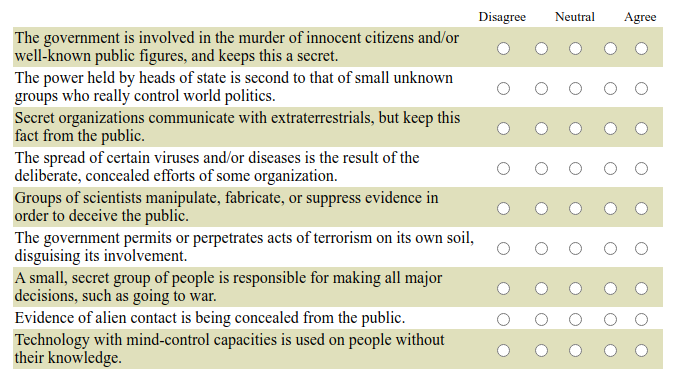
\includegraphics[scale=1.1]{"../survey.png"}\\
\end{center}
The following table contains detailed descriptions of each feature of the dataset.
\newpage
    \begin{tabular}{ c|c }
        Label & Description \\
        \hline
        \textbf{TIPI2} & Question on whether the subject consider themselves \\ & critical and quarrelsome. \\
        \hline
        \textbf{TIPI5} & Question on whether the subject considers themselves \\ & open to new experiences and complex. \\
        \hline
        \textbf{TIPI6} & Question on whether the subject considers themselves \\ & reserved and quiet. \\
        \hline
        \textbf{vocabulary\_misclassification} & All subjects were given a list of 16 words and asked if \\ & they knew what each word meant. 3 of \\ & the words were not real words. So this variable computes \\ & the misclassification rate of only these 3 words to \\ & find people who say they know the definition of a fake word. \\ & This helps us know which people are more \\ & likely to inflate their knowledge. \\
        \hline
        \textbf{STEM} & This is a binary variable saying whether or not \\ & the subject majored in STEM in college. \\
        \hline
        \textbf{education\_2} & Binary variable saying whether the subject only has a \\ & high school education or some other level of education. \\
        \hline
        \textbf{education\_3}  & Binary variable saying whether the subject only has \\ & a University degree or some other level of education. \\
        \hline
        \textbf{urban\_3} & The type of area that the subjects lived in as a child. \\ & This variable is a binary variable showing they either grew \\ & up in an urban environment or not. \\
        \hline
        \textbf{gender\_2} & Binary variable saying whether a subject is female or not. \\
        \hline
        \textbf{engnat\_1} & Binary variable saying whether a subject speaks \\ & English as their native language or not. \\
        \hline
        \textbf{religion\_2} & Binary variable saying whether a subject is \\ & Atheist or not. \\
        \hline
        \textbf{religion\_3} & Binary variable saying whether a subject is \\ & Buddhist or not. \\
        \hline
        \textbf{religion\_7} & Binary variable saying whether a subject is a \\ & non-Catholic, non-LDS, non-Protestant Christian or not. \\
        \hline
        \textbf{religion\_12} & Binary variable saying whether a subject is part \\ & of a religion that is not any major religion. \\
        \hline
        \textbf{orientation\_2} & Binary variable saying whether a subject's \\ & sexual orientation is bisexual or not. \\
        \hline
        \textbf{orientation\_5} & Binary variable saying whether a subject's sexual \\ & orientation is outside of heterosexual, homosexual, \\ & bisexual, and asexual. \\
        \hline
        \textbf{voted\_2} & Binary variable saying whether the subject didn't \\ & vote in the last national election. \\
        \hline
        \textbf{married\_1} & Binary variable saying whether the subject has \\ & never been married. \\
    \end{tabular}
%\newpage
\section*{Data Cleaning and Feature Engineering} The
survey includes many important features including (but not limited to)
age, education, religion, major, and vocabulary comprehension. Most were
categorized and one-hot encoded, but not all. Here we go over the
changes we made in the fields. 
\subsubsection*{GCB - General Conspiracy Belief}
The first field we created was the GCB field, or ``General Conspiracy
Belief''. The first 15 questions of the survey asked about level of
belief in specific conspiracies on a 1-5 scale. The questions were in
the form of statements, like the following example: ``Groups of
scientists manipulate, fabricate, or suppress evidence in order to
deceive the public.'' The GCB is the average of these values for each
person, so 2.5 would indicate an average level of belief of 2.5 in
various conspiracies.

\begin{Shaded}
\begin{Highlighting}[]
\NormalTok{df[}\StringTok{\textquotesingle{}GCB\textquotesingle{}}\NormalTok{] }\OperatorTok{=}\NormalTok{ df[[}\StringTok{\textquotesingle{}Q\textquotesingle{}}\OperatorTok{+}\BuiltInTok{str}\NormalTok{(i) }\ControlFlowTok{for}\NormalTok{ i }\KeywordTok{in} \BuiltInTok{range}\NormalTok{(}\DecValTok{1}\NormalTok{, }\DecValTok{16}\NormalTok{)]].mean(axis}\OperatorTok{=}\DecValTok{1}\NormalTok{) }\OperatorTok{/} \DecValTok{5}
\end{Highlighting}
\end{Shaded}

This was used as the target ``dependent'' variable in our analysis. It
simplifies the regression a lot to use an average of these answers
rather than trying to have 15 different dependent variables.

\hypertarget{major}{%
\subsubsection*{Major}\label{major}}

The last field that we made large changes to was the ``major'' field.
Here, survey respondents would put in their major as a string. Because
this was a free response, we had hundreds of unique responses for major.
Because there are so many majors (and so many major misspellings), we
decided to group the responses together in larger categories. We used
STEM, Humanities, Business/Law, Arts, and Other as our categories.
Logically, this makes sense because we expect majors within the same
sector to have similar correlations to a person's belief in
conspiracies. Because there were such varied responses, we initially
assigned each major to a group manually. We then one-hot encoded these
new variables to facilitate performance of classification. In order to
enable future expansion of the data used, we implemented a flexible
major classification strategy that can sort new major strings robustly
into the existing categories. This strategy uses a Levenshtein edit
distance to find the category with the most similar major in it. This is
calculated with a function that uses recursion to determine the
difference between two strings in terms of how many primitive edits it
takes to permute one into the other. On testing, this strategy worked
quite well and proved to be reliable in categorizing new majors. 
\newline
Below is the code detecting unassigned majors and using the Levenshtein
function to categorize the majors accordingly.

\begin{Shaded}
\begin{Highlighting}[]
\NormalTok{unassigned }\OperatorTok{=}\NormalTok{ df[df[}\StringTok{"STEM"}\NormalTok{]}\OperatorTok{+}\NormalTok{df[}\StringTok{"HUM"}\NormalTok{]}\OperatorTok{+}\NormalTok{df[}\StringTok{"BUS"}\NormalTok{]}\OperatorTok{+}\NormalTok{df[}\StringTok{"OTHER"}\NormalTok{]}\OperatorTok{+}\NormalTok{df[}\StringTok{"ART"}\NormalTok{] }\OperatorTok{==} \DecValTok{0}\NormalTok{]}
\NormalTok{categories }\OperatorTok{=}\NormalTok{ [}\StringTok{"STEM"}\NormalTok{, }\StringTok{"HUM"}\NormalTok{, }\StringTok{"BUS"}\NormalTok{, }\StringTok{"OTHER"}\NormalTok{, }\StringTok{"ART"}\NormalTok{]}
\NormalTok{score }\OperatorTok{=} \BuiltInTok{dict}\NormalTok{()}
\ControlFlowTok{for}\NormalTok{ index,unknown\_string }\KeywordTok{in} \BuiltInTok{zip}\NormalTok{(unassigned.index,unassigned[}\StringTok{\textquotesingle{}major\textquotesingle{}}\NormalTok{]):}
    \ControlFlowTok{for}\NormalTok{ category }\KeywordTok{in}\NormalTok{ categories:}
\NormalTok{        tf }\OperatorTok{=} \BuiltInTok{open}\NormalTok{(}\SpecialStringTok{f"}\SpecialCharTok{\{}\NormalTok{category}\SpecialCharTok{\}}\SpecialStringTok{.txt"}\NormalTok{, }\StringTok{"r"}\NormalTok{,newline}\OperatorTok{=}\StringTok{\textquotesingle{}}\CharTok{\textbackslash{}n}\StringTok{\textquotesingle{}}\NormalTok{)}
\NormalTok{        majors }\OperatorTok{=}\NormalTok{ [i[:}\OperatorTok{{-}}\DecValTok{2}\NormalTok{] }\ControlFlowTok{for}\NormalTok{ i }\KeywordTok{in}\NormalTok{ tf.readlines()]}
\NormalTok{        score[category] }\OperatorTok{=} \BuiltInTok{min}\NormalTok{([levenshteinDistance(}\BuiltInTok{str}\NormalTok{(maj),}\BuiltInTok{str}\NormalTok{(unknown\_string))}\OperatorTok{\textbackslash{}}
\ControlFlowTok{	for}\NormalTok{ maj }\KeywordTok{in}\NormalTok{ majors])}
\NormalTok{    min\_key }\OperatorTok{=} \BuiltInTok{min}\NormalTok{(score, key}\OperatorTok{=}\NormalTok{score.get)}
\NormalTok{    df.loc[index,min\_key] }\OperatorTok{=} \DecValTok{1}
\end{Highlighting}
\end{Shaded}

\hypertarget{vocabulary_knowledge-vocabulary_misclassification}{%
\subsubsection*{Vocabulary Knowledge and
Vocabulary Misclassification}\label{vocabulary_knowledge-vocabulary_misclassification}}

The survey we used included questions in which the respondent identified
the meaning of various vocabulary words. Correct answers for each
question were recorded as 1s, and incorrect as 0s. We did a simple
averaging calculation to determine a person's approximate vocabulary
knowledge (conceivably this works as a very rough proxy for general
lexicographic knowledge). Omitted VCL\_\_ questions were categorized
into a slightly separate variable, since they were nonsense words
included to provide general validity.

\begin{Shaded}
\begin{Highlighting}[]
\NormalTok{df[}\StringTok{\textquotesingle{}validity\textquotesingle{}}\NormalTok{] }\OperatorTok{=}\NormalTok{ df[[}\StringTok{\textquotesingle{}VCL6\textquotesingle{}}\NormalTok{, }\StringTok{\textquotesingle{}VCL9\textquotesingle{}}\NormalTok{, }\StringTok{\textquotesingle{}VCL12\textquotesingle{}}\NormalTok{]].mean(axis}\OperatorTok{=}\DecValTok{1}\NormalTok{)}
knowledge \OperatorTok{=} [1,2,3,4,5,7,8,10,11,13,14,15,16]
\NormalTok{df[}\StringTok{\textquotesingle{}vocabulary\_knowledge\textquotesingle{}}\NormalTok{] }\OperatorTok{=}\NormalTok{ df[[}\StringTok{\textquotesingle{}VCL\textquotesingle{}} \OperatorTok{+} \BuiltInTok{str}\NormalTok{(i) }\ControlFlowTok{for}\NormalTok{ i }\KeywordTok{in}\NormalTok{ knowledge]].mean(axis}\OperatorTok{=}\DecValTok{1}\NormalTok{)}
\end{Highlighting}
\end{Shaded}

\hypertarget{time-feature-engineered}{%
\subsubsection*{Response Time}\label{time-feature-engineered}}

For further feature engineering, we looked at the respondents who took
the least amount of time and the most time to complete the survey, as
well as the respondents who put the same answer for every question on
belief in conspiracy theories. However, upon visual inspection of all of
these edge cases, the demographic information seemed appropriately
varied, and was completely filled out, implying that these rows should
not be thrown out. We concluded that it is likely that the publishers of
this survey data performed similar data cleaning and so any unfinished
surveys or invalid responses would already be thrown out.

%\newpage
\hypertarget{methods}{%
\section*{Methods}\label{methods}}

As mentioned in the introduction, the three methods we compare are $L_1$-regularized least-squares regression, ElasticNet regression, and a Random Forest ensemble of regression trees. We first use least-squares regression with \(L_1\)-regularization, hoping to remove any irrelevant features.
We use $\alpha=1\times10^{-3}$, which reduces
the 100+ columns down to the 20 columns with nonzero
coefficients. We then run OLS without any regularization on the reduced set
of columns so that the results won't include features with coefficients of zero. The next methods we use are ElasticNet and Random Forest regression. In both
cases we used a grid search across various hyperparameters, illustrated in Table~\ref{tab:hyper} with 5-way cross validation looking to
maximize the classifier's \(R^2\) value. With the Random Forests, we
limited the possible tree parameters to preclude overfitting. In fact,
by letting the max tree depth be 10, we found the tree to have an
\(R^2\) value of over .5, much higher than the \(.15\)-\(.2 R^2\) values
found by the OLS estimators. We concluded that the forest was likely
very overfit, and so restricted ourselves to more conservative hyper
parameters. 
\newpage
\section*{Results}
For our initial attempt using \(L_1\)-regularization, the figure below
shows the coefficient of determination \(R^2\) and correlation
coefficients for different features.
\begin{center}
\begin{tabular}{lclc}
\toprule
\textbf{Dep. Variable:}                &       GCB        & \textbf{  R-squared:         } &     0.135   \\
\textbf{Model:}                        &       OLS        & \textbf{  Adj. R-squared:    } &     0.129   \\
\textbf{Method:}                       &  Least Squares   & \textbf{  F-statistic:       } &     24.15   \\
\textbf{Date:}                         & Wed, 01 Dec 2021 & \textbf{  Prob (F-statistic):} &  8.15e-67   \\
\textbf{Time:}                         &     17:11:36     & \textbf{  Log-Likelihood:    } &    573.41   \\
\textbf{No. Observations:}             &        2495      & \textbf{  AIC:               } &    -1113.   \\
\textbf{Df Residuals:}                 &        2478      & \textbf{  BIC:               } &    -1014.   \\
\textbf{Df Model:}                     &          16      & \textbf{                     } &             \\
\textbf{Covariance Type:}              &    nonrobust     & \textbf{                     } &             \\
\bottomrule
\end{tabular}
\begin{tabular}{lcccccc}
                                       & \textbf{coef} & \textbf{std err} & \textbf{t} & \textbf{P$> |$t$|$} & \textbf{[0.025} & \textbf{0.975]}  \\
\midrule
\textbf{TIPI1}                         &       0.0046  &        0.003     &     1.817  &         0.069        &       -0.000    &        0.010     \\
\textbf{TIPI2}                         &       0.0130  &        0.002     &     5.968  &         0.000        &        0.009    &        0.017     \\
\textbf{TIPI5}                         &       0.0038  &        0.003     &     1.321  &         0.187        &       -0.002    &        0.009     \\
\textbf{TIPI6}                         &       0.0003  &        0.003     &     0.101  &         0.919        &       -0.005    &        0.005     \\
\textbf{TIPI7}                         &       0.0013  &        0.002     &     0.541  &         0.589        &       -0.003    &        0.006     \\
\textbf{vocabulary\_misclassification} &       0.0707  &        0.017     &     4.045  &         0.000        &        0.036    &        0.105     \\
\textbf{OTHER}                         &       0.0228  &        0.008     &     2.699  &         0.007        &        0.006    &        0.039     \\
\textbf{education\_2}                  &       0.0301  &        0.008     &     3.637  &         0.000        &        0.014    &        0.046     \\
\textbf{urban\_3}                      &       0.0237  &        0.008     &     2.890  &         0.004        &        0.008    &        0.040     \\
\textbf{gender\_2}                     &       0.0229  &        0.008     &     2.880  &         0.004        &        0.007    &        0.039     \\
\textbf{religion\_2}                   &      -0.0756  &        0.009     &    -8.253  &         0.000        &       -0.094    &       -0.058     \\
\textbf{religion\_3}                   &       0.0864  &        0.028     &     3.092  &         0.002        &        0.032    &        0.141     \\
\textbf{religion\_7}                   &       0.0639  &        0.014     &     4.449  &         0.000        &        0.036    &        0.092     \\
\textbf{religion\_12}                  &       0.1034  &        0.013     &     8.256  &         0.000        &        0.079    &        0.128     \\
\textbf{orientation\_5}                &       0.0438  &        0.017     &     2.591  &         0.010        &        0.011    &        0.077     \\
\textbf{voted\_2}                      &       0.0208  &        0.009     &     2.434  &         0.015        &        0.004    &        0.038     \\
\textbf{const}                         &       0.4135  &        0.028     &    14.870  &         0.000        &        0.359    &        0.468     \\
\bottomrule
\end{tabular}
\begin{tabular}{lclc}
\textbf{Omnibus:}       & 76.163 & \textbf{  Durbin-Watson:     } &    1.910  \\
\textbf{Prob(Omnibus):} &  0.000 & \textbf{  Jarque-Bera (JB):  } &   40.646  \\
\textbf{Skew:}          &  0.123 & \textbf{  Prob(JB):          } & 1.49e-09  \\
\textbf{Kurtosis:}      &  2.425 & \textbf{  Cond. No.          } &     80.3  \\
\bottomrule
\end{tabular}
%\caption{OLS Regression Results}
\end{center}

Notes: \newline
 [1] Standard Errors assume that the covariance matrix of the errors is
correctly specified.

None of our features seems to be strongly correlated with GCB, and we
only account for about 13.9\% of the variance in beliefs with these
features. Among what we did find, however, the strongest predictors of
belief in conspiracy theories seem to be religion (in particular marking
`other' as one's choice of religion), low knowledge of the given
vocabulary words, and age. The engineered features ``vocabulary
knowledge'' and ``vocabulary\_misclassification'' determine this.

We got better results using a grid search on the sklearn implementations
of ElasticNet and RandomForestRegressor. As can be seen in the below
table, we got our best results using a random forest with an \(R^2\) of
.2297, much better than the .135 than plain OLS. Note that the random
forest listed here is not the best (in terms of \(R^2\)) random forest
that we were able to generate, but it is the best that has hyper
parameters that don't lend themselves to overfitting.

%\begin{center}
%\captionof{table}{Table 1: Best Hyperparameters from Grid Search.}
\begin{table}[ht]
	\centering
	\caption{Best Hyperparameters.} \label{tab:hyper} 
	\vspace{10mm}
\begin{tabular}{ |c|c|c| } 
       \hline
       Model & Best Hyperparameters & $R^2$ \\ 
       \hline
       sklearn ElasticNet & $\alpha = .001$, \verb|l1_ratio| $= .4842$ & .1811 \\ 
       sklearn RandomForestRegressor & \verb|max_depth| = 5, \verb|min_samples_leaf| = 6 & .2297 \\
       \hline
	\end{tabular}
\end{table}
%\end{center}

In the next table, we see which features were most impactful in the
Random Forest. Note that a high gini importance indicates that a feature
is important in determining whether or not a person believes in
conspiracy theories, but that feature is not necessarily positively
correlated (it could be negatively correlated). The way the OLS
regression interpreted these features, religion\_2,
vocabulary\_knowledge, and TIPI10 were negatively correlated, and
religion\_12 and age were positively correlated.

\begin{center}
\begin{tabular}{ |c|c|c| } 
   \hline
   Column & Meaning & Gini Importance \\ 
   \hline
   \verb|religion_2| & Atheist & .2040 \\ 
   \verb|vocabulary_knowledge| & \% of words marked correctly & .1749 \\ 
   \verb|religion_12| & "Other" Religion & .1218 \\ 
   \verb|age| & Years Old & .0664 \\ 
   \verb|TIPI10| & Conventional, Uncreative Personality & .0566 \\ 
   \hline
\end{tabular}
\end{center}

By analyzing this data we found that among the group of people that was
surveyed, there are a number of features which are definitely correlated
with belief in conspiracy theories. These features are definitely
correlated among the group of survey respondents, and it is possible
that these features could also be very gently correlated with conspiracy
belief in the population in general. However, it is important to note
that 1) our \(R^2\) values indicate that our model accounts for very
little variation of belief in conspiracy beliefs and 2) since this was
an online volunteer survey, we have no reason to believe that the
respondents are representative of society or any general group.

None of our features seems to be strongly correlated with GCB, and we only account for about 13.9$\%$ of the variance in beliefs with these features. Among what we did find, however, the strongest predictors of belief in conspiracy theories seem to be religion (in particular marking ‘other’ as one’s choice of religion), low knowledge of the given vocabulary words, and age. The engineered features "vocabulary knowledge" and "vocabulary\_misclassification" indicate the knowledge of vocab words, and age is a quasi-continuous variable. The following figure is a heatmap of General Conspiracy Belief in relation to a person’s age and vocabulary score. Although we do see a concentration of higher GCB in the lower age/lower vocab score area, there is no strong correlation immediately apparent. This matches up with the low predictive power of our various regressors - correlations do exist, but are not strong.
\begin{center}
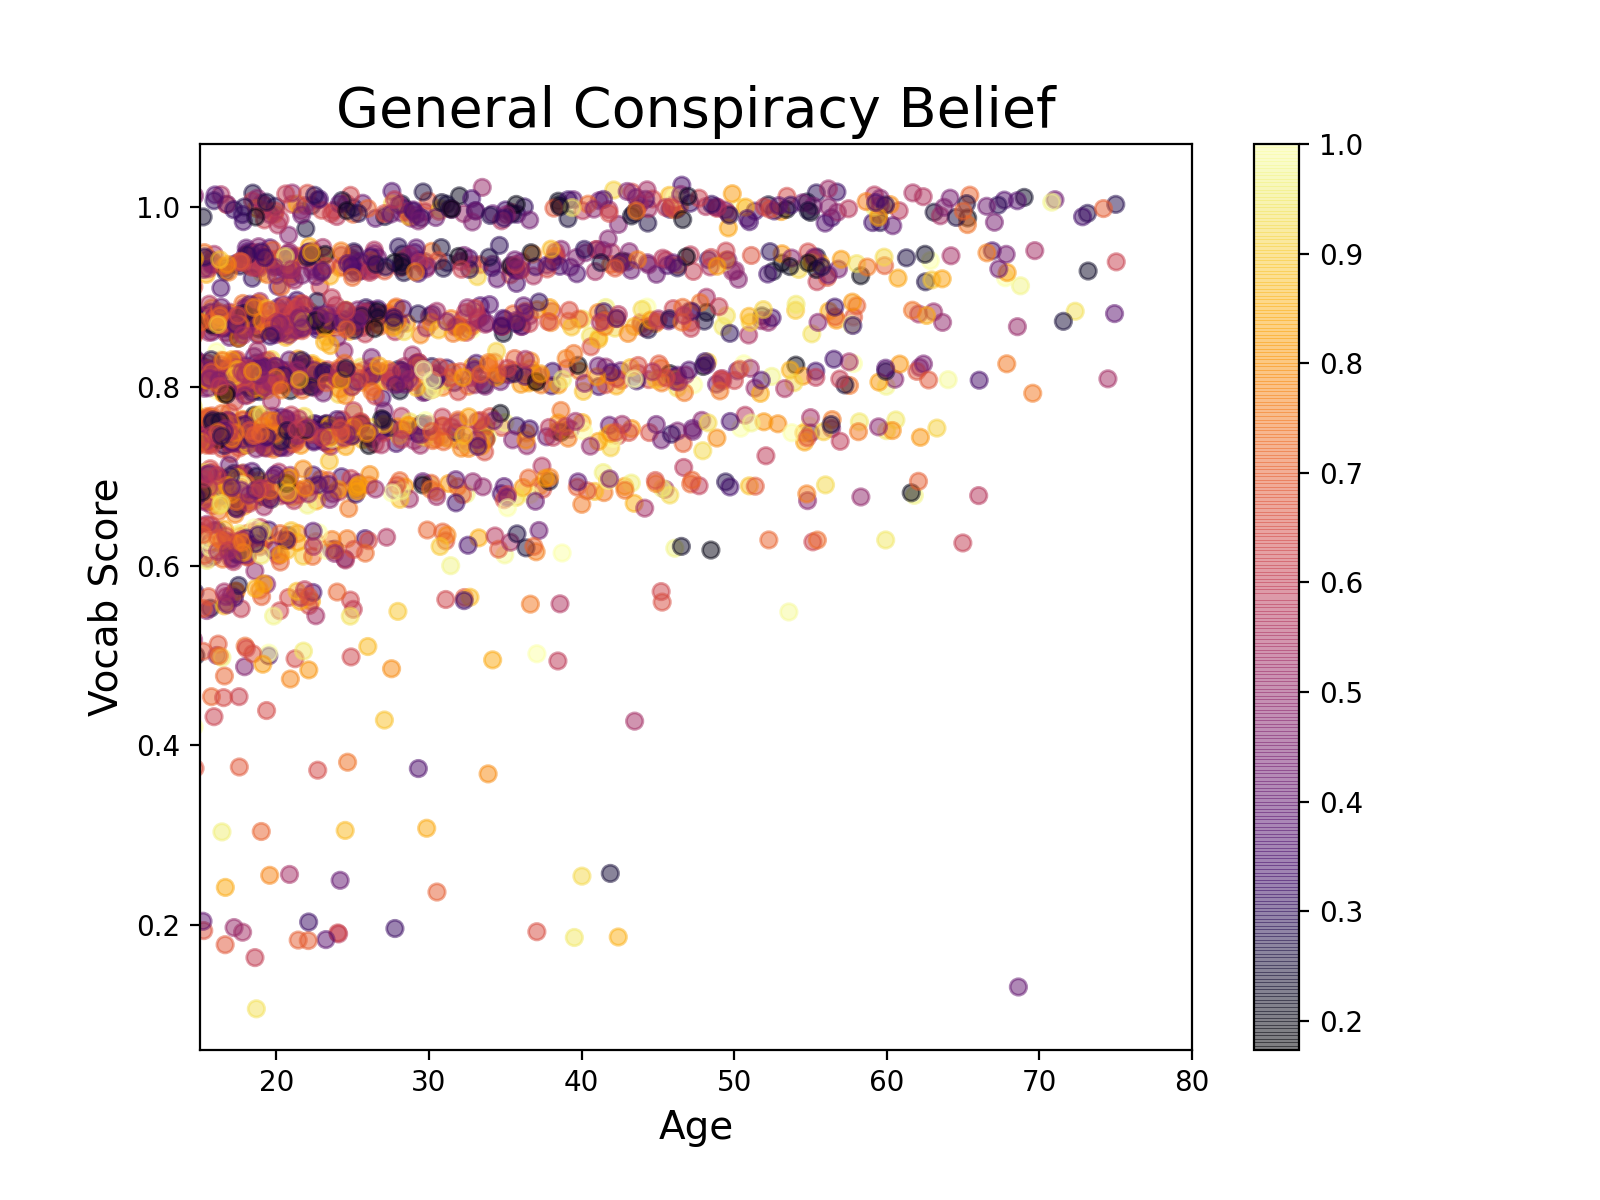
\includegraphics[scale=1.2]{"../VocabAge_GCB.png"}
\end{center}
%\newpage
    \hypertarget{ethical-implications}{%
\section*{Ethical Implications}\label{ethical-implications}}

It is important to remember that, although we have found traits with
positive and negative correlation to conspiracy theory belief, our model
has a very low R\^{}2 score. That means that our model does not account
for a lot of the variance in the data. Thus, just because someone may
have many of the traits that correlate with conspiracy theory belief,
that does not mean they do believe in conspiracy theories. Human beings
are diverse and multi-faceted in their beliefs. Thus, absolute
assumptions should not be made from the data above. Instead, the data
above should be used as merely a soft guide to indicate that a person
may believe conspiracy theories. This could be useful in anticipating a
group's beliefs prior to giving them information about controversial
topics, or in determining the issues most important to a group of
people. But again, it should not be used to make absolute assumptions.
Additionally, it is important that predictions from this model not be
used to discriminate against individuals or disqualify them from
anything, such as jobs or political offices. High correlations are good
leads for other questions of research, such as ``why is belief in
conspiracy highly correlated with \_\_\_\_?'' Understanding the causes
behind the trends could help us answer questions about nature
vs.~nurture, psychology, and other topics in the field of study.

\newpage
\hypertarget{references}{%
\section*{References}\label{references}}
\begin{enumerate}
\item Bowes, S. M., Costello, T. H., Ma, W., \& Lilienfeld, S. O. (2021).
Looking under the tinfoil hat: Clarifying the personological and
psychopathological correlates of conspiracy beliefs. Journal of
Personality, 89(3), 422-436.
\newline\url{https://doi.org/https://doi.org/10.1111/jopy.12588}

\item Galliford, N., \& Furnham, A. (2017). Individual difference factors and beliefs in medical
and political conspiracy theories. Scandinavian Journal of Psychology,
58(5), 422-428. \newline\url{https://doi.org/https://doi.org/10.1111/sjop.12382}

\item Brotherton, R., French, C. C., \& Pickering, A. D. (2013). Measuring belief in conspiracy theories: The generic conspiracist beliefs scale. Frontiers in Psychology, 4, 279. \newline\url{https://doi.org/10.3389/fpsyg.2013.00279}

\end{enumerate}


    % Add a bibliography block to the postdoc
    
    
    
\end{document}
